\documentclass{article}
\usepackage[utf8]{inputenc}
\usepackage{graphicx}
\usepackage{ragged2e}
\usepackage[margin=2.5cm]{geometry}
\usepackage{array}
\usepackage{wrapfig}
\usepackage{multirow}
\usepackage{tabularx}
\usepackage{amsmath}
\usepackage{wrapfig}
\usepackage{enumitem }
\usepackage{mathtools}
\usepackage[table]{xcolor}
\usepackage{multirow}
\usepackage{polski}
\usepackage{enumitem}
\usepackage{rotating}
\usepackage{natbib}
\usepackage{matlab-prettifier}
\usepackage{graphicx}
\usepackage[dvipsnames]{xcolor}
\usepackage{amssymb}
\usepackage[export]{adjustbox}
\title{Sprawozdanie 6}
\author{AUTOR}
\date{}

\newcommand{\inv}{^{\raisebox{.2ex}{$\scriptscriptstyle-1$}}}
\begin{document}

\maketitle

\section{Cel ćwiczenia}
Poznanie własności podstawowych członów dynamiki. Nabycie umiejętności wyznaczania parametrów transmitancji na podstawie otrzymanego wykresu.


\section{Schematy symulacyjne}
%%%%%%%%%%%%%%%%%%%%%%%%%%%%%%%%%%%%%%%%%%%%%%%%%%%%
Człon inercyjny:
$$
\frac{K}{(T_{1}s+1)(T_{2}s+1)}
$$
% model 1
$T_{1}, T_{2}$ - stałe czasowe\\
$K=2$ - wzmocnienie członu\\
$T_{1}=1$
\begin{enumerate}[label=\alph*)]
\item $T_{2}=0$
\item $T_{2}=T_{1}/10$
\item $T_{2}=T_{1}/2$
\item $T_{2}=T_{1}\cdot 1.05$
\end{enumerate}{}

\begin{figure}[h!]
    \centering
    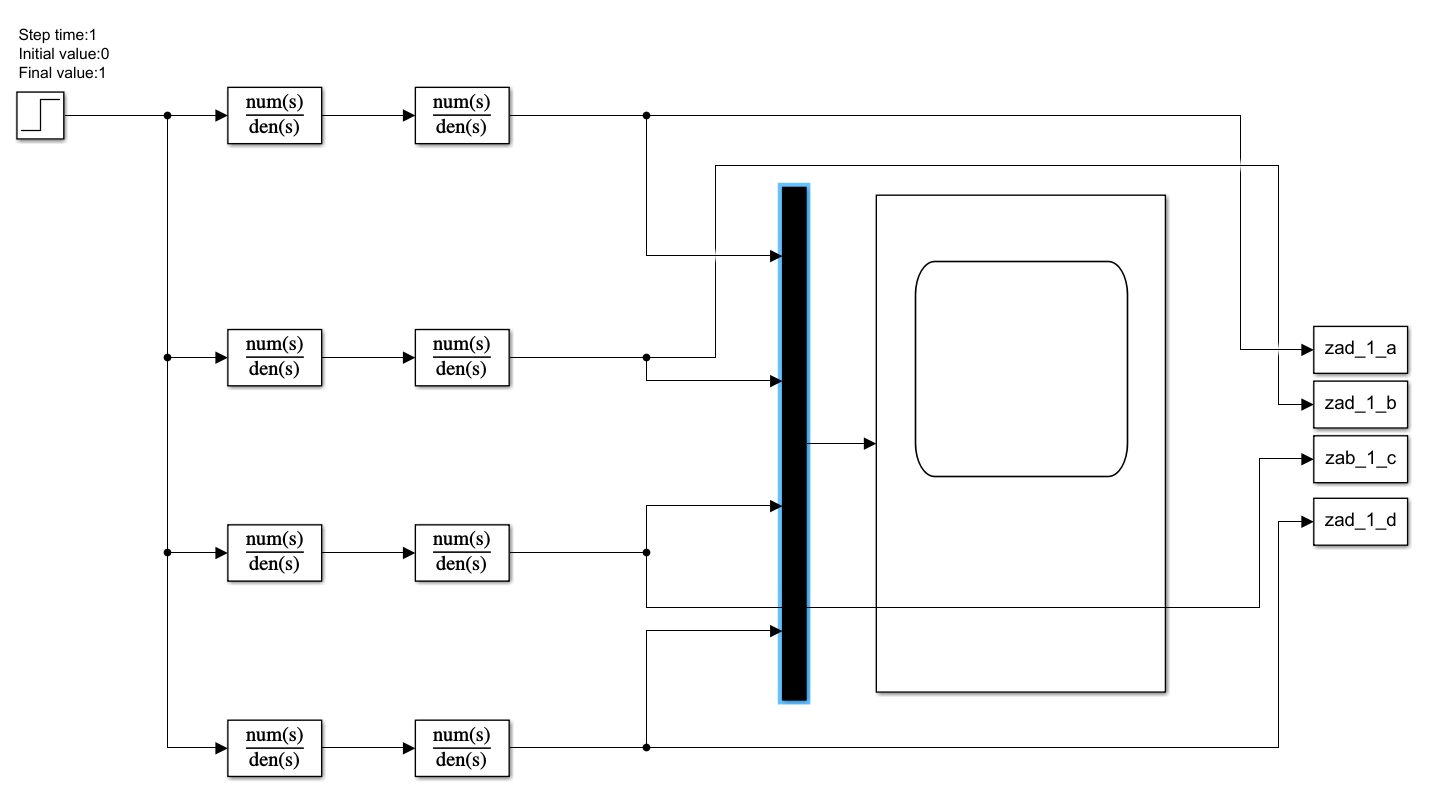
\includegraphics[scale=0.4]{model_inercyjny.png}
    \caption{Schemat modelu inercyjnego}
    \label{fig:model_inercyjny}
\end{figure}
\newpage
%%%%%%%%%%%%%%%%%%%%%%%%%%%%%%%%%%%%%%%%%%%%%%%%%%%%
\begin{flushleft}

Człon całkujący:
\end{flushleft}{}
$$
\frac{K}{T_{i}s(T_{2}+1)}
$$
% model 2

$T_{2}$ - stała czasowa\\
$K=2$ - wzmocnienie członu\\
$T_{i}=1$ - czas całkowania\\
\begin{enumerate}[label=\alph*)]
\item $T_{2}=0$ \ (całk. idealny)
\item $T_{2}=T_{i}/100$\ (całk. rzeczywisty)
\item $T_{2}=T_{i}/10$
\item $T_{2} \approx T_{i}$
\item $T_{2}=T_{i}\cdot 10$
\end{enumerate}

\begin{figure}[h!]
    \centering
    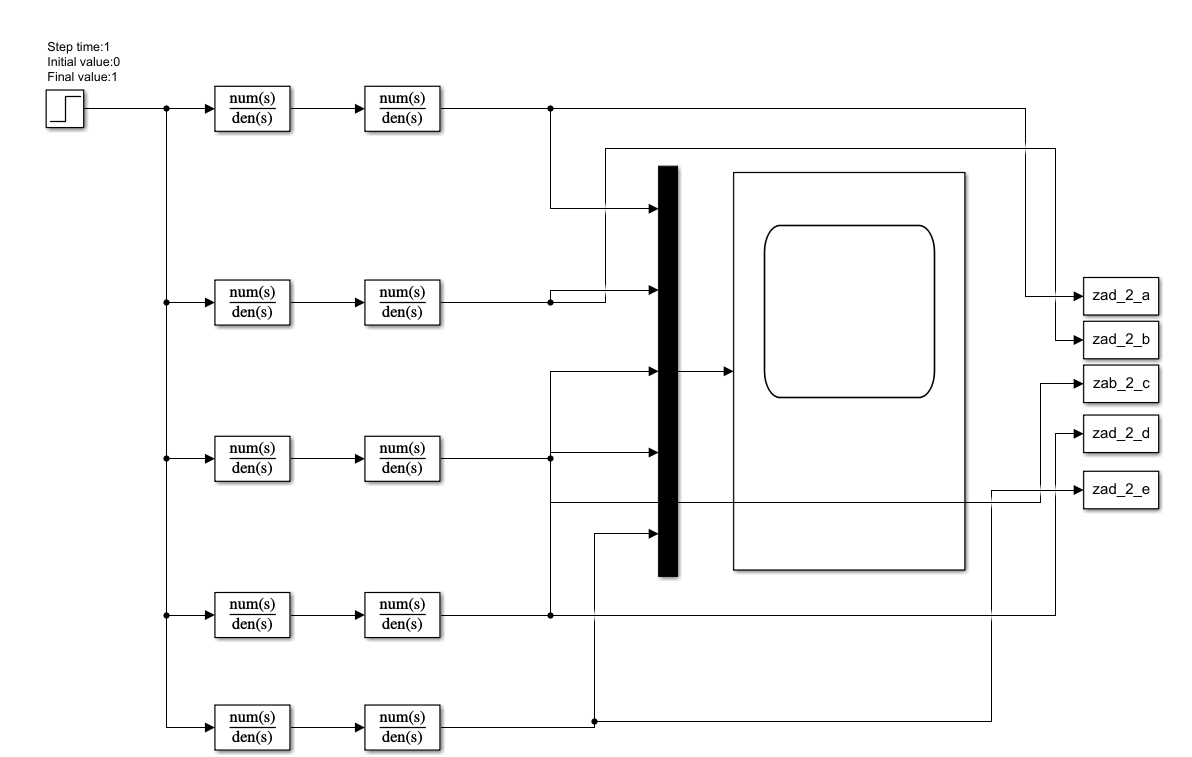
\includegraphics[scale=0.6]{model_calkujacy.png}
    \caption{Schemat modelu całkującego}
    \label{fig:model_calkujacy}
\end{figure}
\newpage
%%%%%%%%%%%%%%%%%%%%%%%%%%%%%%%%%%%%%%%%%%%%%%%%%%%%
\begin{flushleft}

Człon różniczkujący:
\end{flushleft}{}

$$
\frac{T_{d}s}{(T_{2}s+1)}
$$
% model 3

$T_{2}$ - stała czasowa\\
$K=2$ - wzmocnienie członu\\
$T_d=1$ - czas różiczkowania\\
\begin{enumerate}[label=\alph*)]
\item $T_{2}=0$ \ (różn. idealny)
\item $T_{2}=T_{d}/100$\ (różn. rzeczywisty)
\item $T_{2}=T_{d}/10$
\item $T_{2} \approx T_{d}$
\item $T_{2}=T_{d}\cdot 10$
\end{enumerate}{}

\begin{figure}[h!]
    \centering
    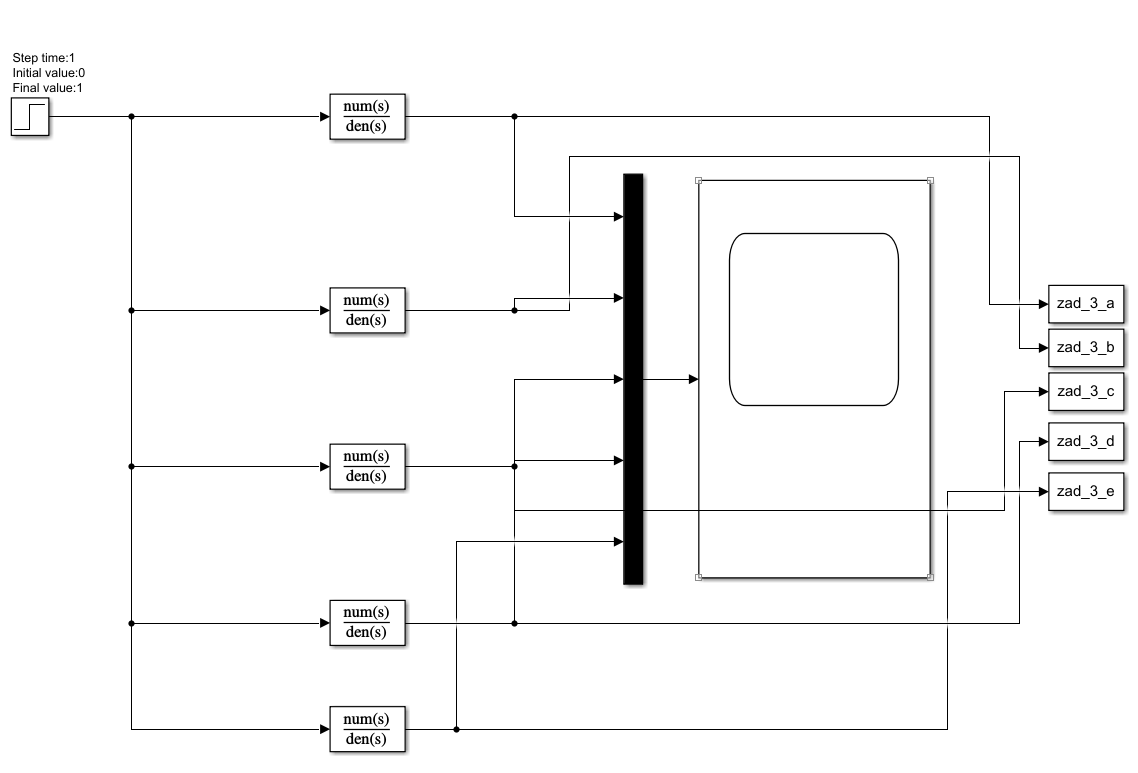
\includegraphics[scale=0.6]{model_rozniczkujacy.png}
    \caption{Schemat modelu różniczkującego}
    \label{fig:model_rozniczkujacego}
\end{figure}
%%%%%%%%%%%%%%%%%%%%%%%%%%%%%%%%%%%%%%%%%%%%%%%%%%%%
\newpage

Aby móc uzyskać symulacje przybliżono wartość $T_{2}=0$ do $T_{2}=0.0001$, dla członu różniczkującego.
Otrzymane wyniki symulacji dla poszczególnych członów:\\
Członu inercyjnego:
\begin{figure}[h!]
    \centering
    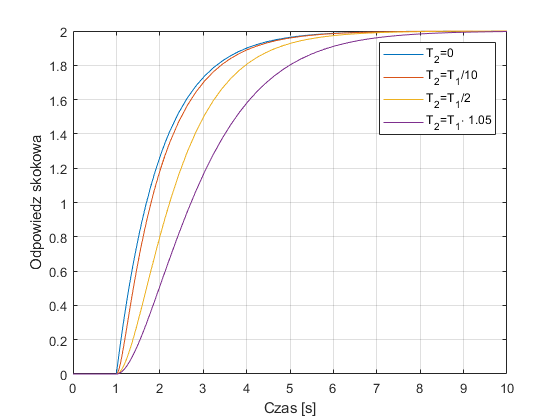
\includegraphics[scale=0.5]{all_inercyjny.png}
    \caption{Wszystkie symulacje członu inercyjnego}
    \label{fig:all_inercyjny}
\end{figure}

\vspace{-2ex}

Członu całkującego:
\begin{figure}[h!]
    \centering
    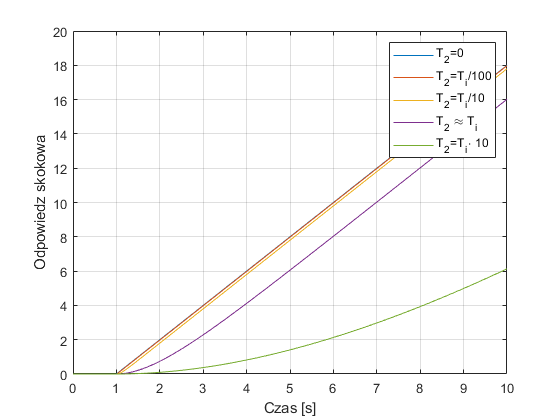
\includegraphics[scale=0.5]{all_calkujacy.png}
    \caption{Wszystkie symulacje członu całkującego}
    \label{fig:all_calkujacy}
\end{figure}


\vspace{-2ex}

Członu różniczkującego:
\begin{figure}[h!]
    \centering
    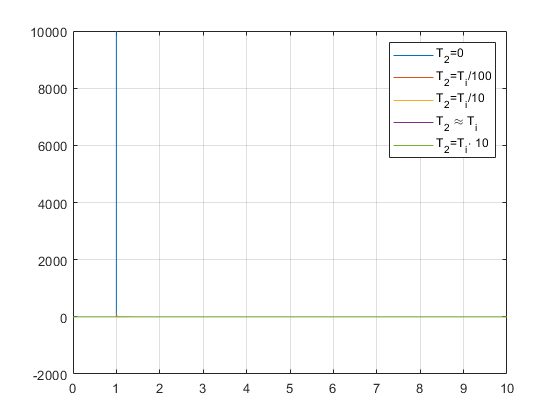
\includegraphics[scale=0.5]{all_rozniczkujacy.png}
    \caption{Wszystkie symulacje członu różniczkującego}
    \label{fig:all_rozniczkujacy}
\end{figure}


%%%%%%%%%%%%%%%%%%%%%%%%%%%%%%%%%%%%%%%%%%%%%%%%%%%%
\newpage
Poszczególne wykresy członu różniczkującego:

\begin{figure}[h!]
    \centering
    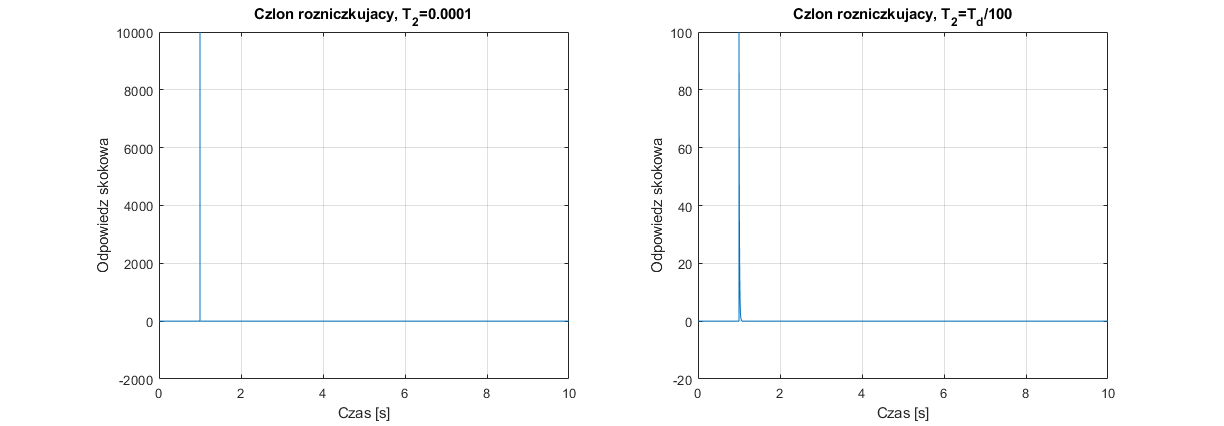
\includegraphics[scale=0.5]{roz_1_2.png}

    \label{fig:my_label}
\end{figure}{}

\begin{figure}[h!]
    \centering
    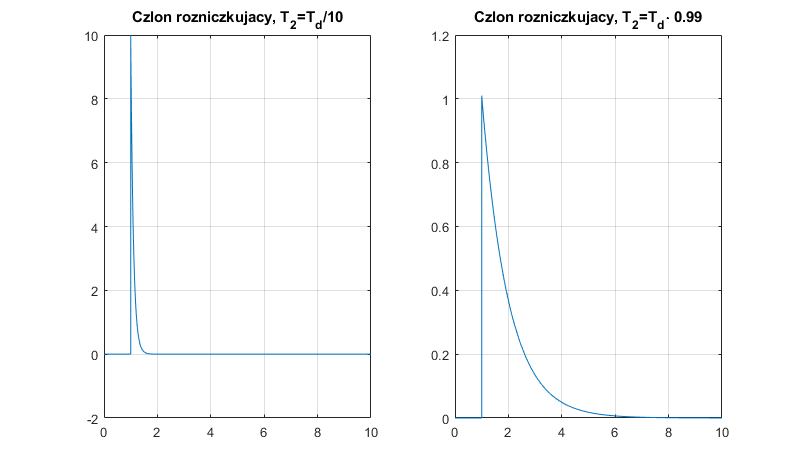
\includegraphics[scale=0.5]{roz_3_4.png}

    \label{fig:my_label}
\end{figure}{}

\begin{figure}[h!]
    \centering
    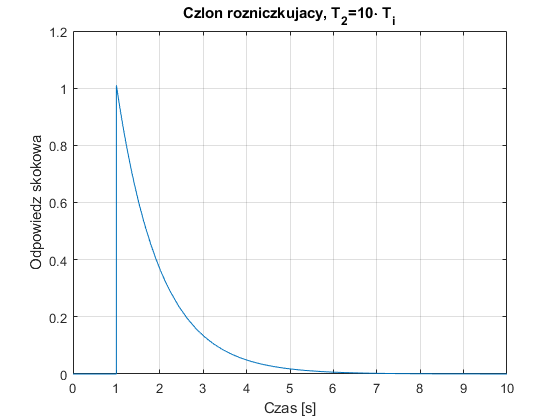
\includegraphics[scale=0.5]{roz_6.png}
    \label{fig:my_label}
\end{figure}{}
%%%%%%%%%%%%%%%%%%%%%%%%%%%%%%%%%%%%%%%%%%%%%%%%%%%%
\newpage
Poszczególne wykresy członu inercyjnego:

\begin{figure}[h!]
\hspace{-5cm}
    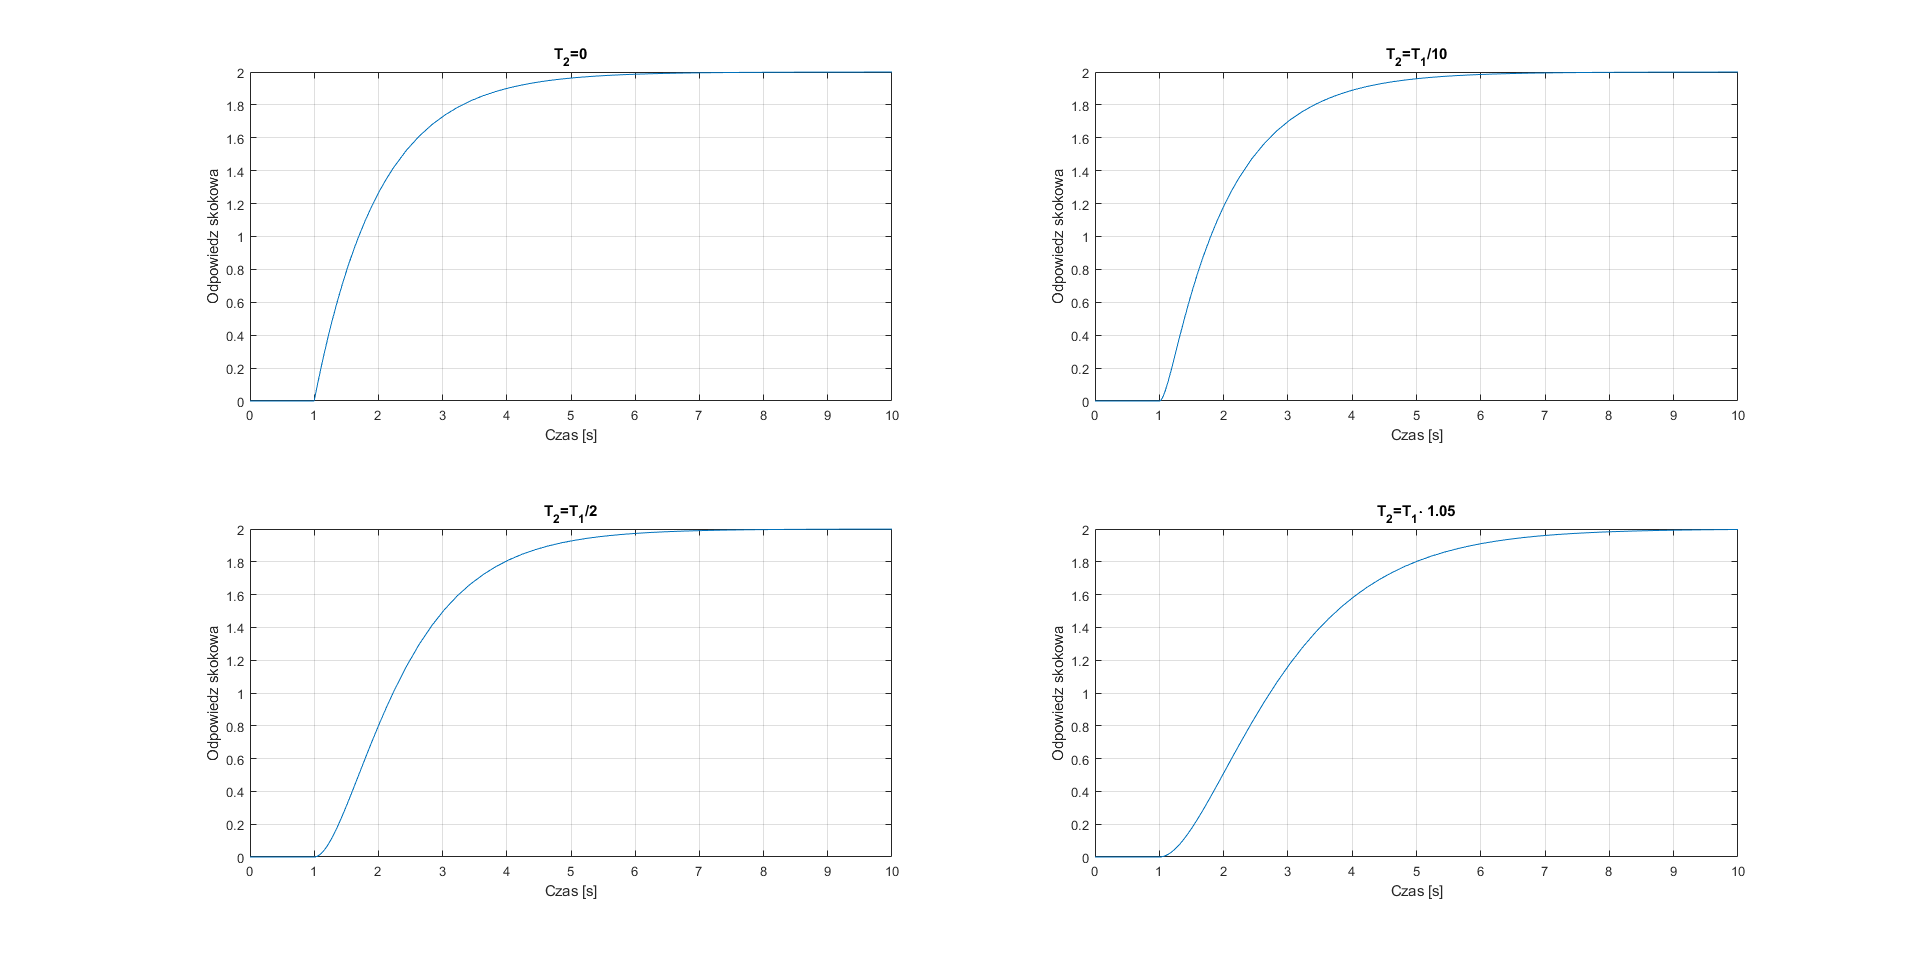
\includegraphics[scale=0.5]{inerc_a_b_c_d.png}
    \label{fig:each_iner}
\end{figure}{}


%trzeba dac pojedyncze inercyjnego zeby na nich rysowac
\newpage
%%%%%%%%%%%%%%%%%%%%%%%%%%%%%%%%%%%%%%%%%%%%%%%%%%%%
\section{Metoda Kumpfmüllera}

Model, dla odczytanych członów Kumpfmüllera:

\begin{figure}[h!]
    \centering
    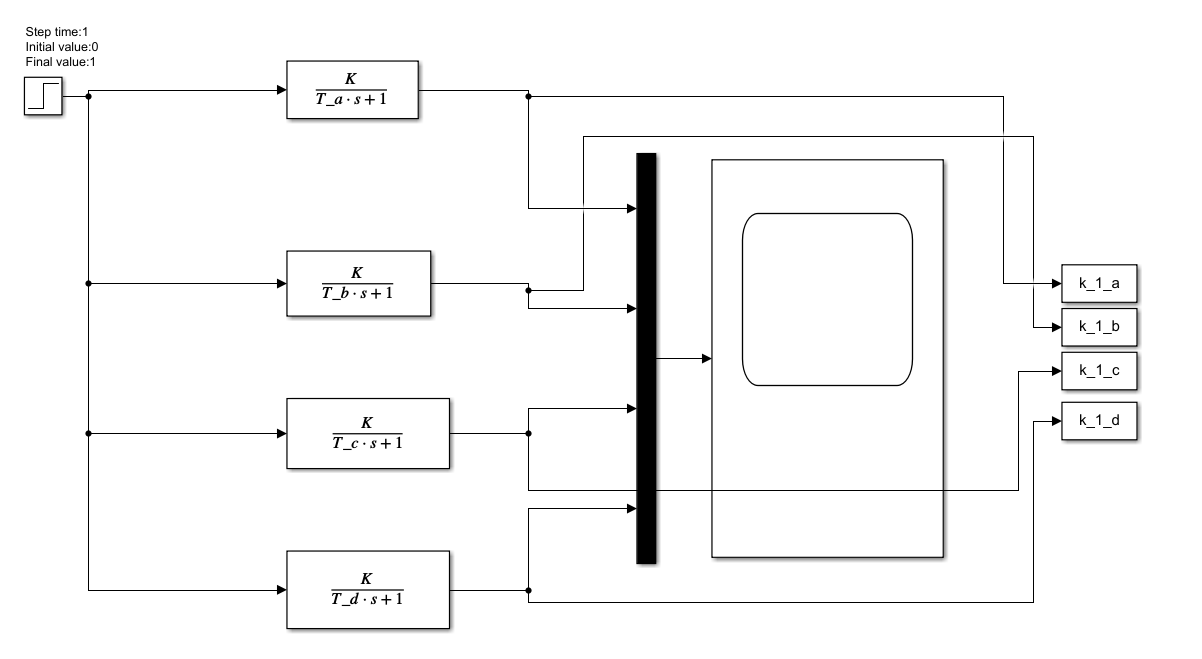
\includegraphics[scale=0.5]{model_kumpf.png}
    \label{fig:my_label}
\end{figure}{}


\newpage
%%%%%%%%%%%%%%%%%%%%%%%%%%%%%%%%%%%%%%%%%%%%%%%%%%%%
Porównanie odpowiedzi skokowych członów inercyjnych zadanych podczas zajęć z członami otrzymanymi za pomocą metodą Kumpfmüllera:
\begin{figure}[h!]
\hspace{-5cm}
    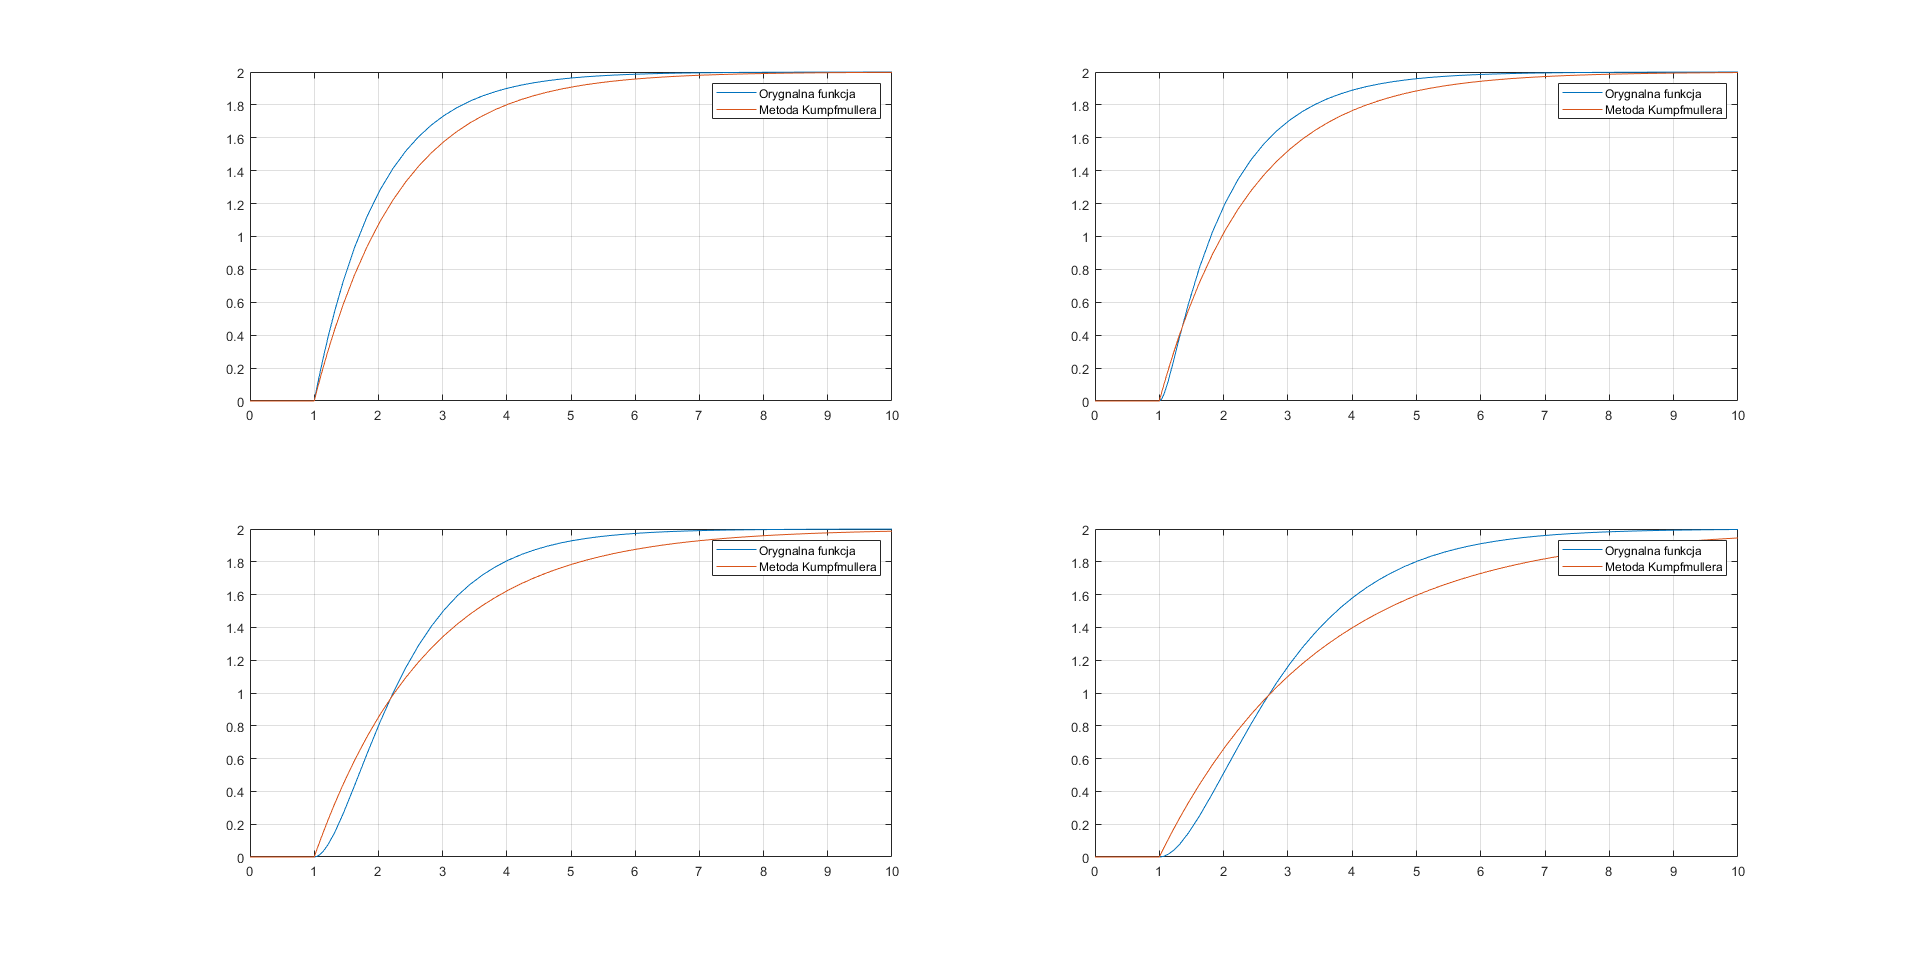
\includegraphics[scale=0.5]{kumpf_inerc_a_b_c_d.png}
    \label{fig:each_iner}
\end{figure}{}


Odczytane wartości:
\begin{enumerate}[label=\alph*)]
\item[] $K=2$
\item $T=1.3$
\item $T=1.4$
\item $T=1.8$  
\item $T=2.5$
\end{enumerate}{}


%%%%%%%%%%%%%%%%%%%%%%%%%%%%%%%%%%%%%%%%%%%%%%%%%%%%

\section{Wnioski}

Dla członu inercyjnego, przy $T_{2}=0$ układ stabilizuje się najszybciej. Im większa wartość $T_{2}$ tym układ dłużej się stabilizuje. Dla członu całkującego przebieg $T_{2}=0$ od początku ma formę funkcji liniowej. Jest to idealny człon całkujący. Im większe $T_{2}$ tym potrzeba więcej czasu potrzeba, aby przebieg przypominał funkcje liniową. Dla członu różniczkującego $T_{2}$ dążące do 0 najbardziej przypomina impuls. Jest to w przybliżeniu idealny człon różniczkujący. Im większe $T_{2}$ tym funkcja osiąga niższe wartości oraz dłużej się stabilizuje.

\newpage


\section{Załącznik}


\begin{lstlisting}[style=Matlab-editor]


clear;
close all;


K=2;

% model 1

T_1=1;

T_1_a=0;
T_1_b=T_1/10;
T_1_c=T_1/2;
T_1_d=T_1*1.05;

% model 2

T_i=1;

T_2_a=0;
T_2_b=T_i/100;
T_2_c=T_i/10;
T_2_d=T_i*0.99;
T_2_e=10*T_i;


% model 3

T_d=1;

T_3_a=0.0001;
T_3_b=T_d/100;
T_3_c=T_d/10;
T_3_d=T_d*0.99;
T_3_e=10*T_i;

%%%%%%%%%%%%%%%%%%%%%%%%%%%%%%%%%%%%%%%%%
sim('transmitancje_lab10')
% Rysowanie INERCYJNY
figure(1);
plot(zad_1_a)
hold on;
plot(zad_1_b)
hold on;
plot(zad_1_c)
hold on;
plot(zad_1_d)
grid on;
xlabel("Czas [s]")
ylabel("Odpowiedz skokowa")

legend('T_{2}=0','T_{2}=T_{1}/10','T_{2}=T_{1}/2','T_{2}=T_{1}\cdot 1.05')

%%%%%%%%%%%%%%%%%%%%%%%%%%%%%%%%%%%%%%%%%
% Rysowanie Calkujacy

figure(2);
plot(zad_2_a)
hold on;
plot(zad_2_b)
hold on;
plot(zad_2_c)
hold on;
plot(zad_2_d)
hold on;
plot(zad_2_e)
grid on;
xlabel("Czas [s]")
ylabel("Odpowiedz skokowa")

legend('T_{2}=0','T_{2}=T_{i}/100','T_{2}=T_{i}/10','T_{2} \approx T_{i}','T_{2}=T_{i}\cdot 10')

%%%%%%%%%%%%%%%%%%%%%%%%%%%%%%%%%%%%%%%%%
% Rysowanie ROZNICZKUJACY

figure(3);
plot(zad_3_a)
hold on;
plot(zad_3_b)
hold on;
plot(zad_3_c)
hold on;
plot(zad_3_d)
hold on;
plot(zad_3_e)
grid on;
legend('T_{2}=0','T_{2}=T_{i}/100','T_{2}=T_{i}/10','T_{2} \approx T_{i}','T_{2}=T_{i}\cdot 10')
xlabel("Czas [s]")
ylabel("Odpowiedz skokowa")

% ROZNICZKUJACY OSOBNO

figure(4);
subplot(121)
plot(zad_3_a)
grid on;
title("Czlon rozniczkujacy, T_{2}=0.0001")
xlabel("Czas [s]")
ylabel("Odpowiedz skokowa")



\end{lstlisting}




\end{document}



















